%% bare_conf.tex
%% V1.4
%% 2012/12/27
%% by Michael Shell
%% See:
%% http://www.michaelshell.org/
%% for current contact information.
%%
%% This is a skeleton file demonstrating the use of IEEEtran.cls
%% (requires IEEEtran.cls version 1.8 or later) with an IEEE conference paper.
%%
%% Support sites:
%% http://www.michaelshell.org/tex/ieeetran/
%% http://www.ctan.org/tex-archive/macros/latex/contrib/IEEEtran/
%% and
%% http://www.ieee.org/

%%*************************************************************************
%% Legal Notice:
%% This code is offered as-is without any warranty either expressed or
%% implied; without even the implied warranty of MERCHANTABILITY or
%% FITNESS FOR A PARTICULAR PURPOSE! 
%% User assumes all risk.
%% In no event shall IEEE or any contributor to this code be liable for
%% any damages or losses, including, but not limited to, incidental,
%% consequential, or any other damages, resulting from the use or misuse
%% of any information contained here.
%%
%% All comments are the opinions of their respective authors and are not
%% necessarily endorsed by the IEEE.
%%
%% This work is distributed under the LaTeX Project Public License (LPPL)
%% ( http://www.latex-project.org/ ) version 1.3, and may be freely used,
%% distributed and modified. A copy of the LPPL, version 1.3, is included
%% in the base LaTeX documentation of all distributions of LaTeX released
%% 2003/12/01 or later.
%% Retain all contribution notices and credits.
%% ** Modified files should be clearly indicated as such, including  **
%% ** renaming them and changing author support contact information. **
%%
%% File list of work: IEEEtran.cls, IEEEtran_HOWTO.pdf, bare_adv.tex,
%%                    bare_conf.tex, bare_jrnl.tex, bare_jrnl_compsoc.tex,
%%                    bare_jrnl_transmag.tex
%%*************************************************************************

% *** Authors should verify (and, if needed, correct) their LaTeX system  ***
% *** with the testflow diagnostic prior to trusting their LaTeX platform ***
% *** with production work. IEEE's font choices can trigger bugs that do  ***
% *** not appear when using other class files.                            ***
% The testflow support page is at:
% http://www.michaelshell.org/tex/testflow/



% Note that the a4paper option is mainly intended so that authors in
% countries using A4 can easily print to A4 and see how their papers will
% look in print - the typesetting of the document will not typically be
% affected with changes in paper size (but the bottom and side margins will).
% Use the testflow package mentioned above to verify correct handling of
% both paper sizes by the user's LaTeX system.
%
% Also note that the "draftcls" or "draftclsnofoot", not "draft", option
% should be used if it is desired that the figures are to be displayed in
% draft mode.
%
\documentclass[conference]{IEEEtran}
% Add the compsoc option for Computer Society conferences.
%
% If IEEEtran.cls has not been installed into the LaTeX system files,
% manually specify the path to it like:
% \documentclass[conference]{../sty/IEEEtran}



% Some very useful LaTeX packages include:
% (uncomment the ones you want to load)


% For directly writing german umlauts uncomment the appropriate line for
% your operating system:
% Windows:
% \usepackage[ansinew]{inputenc}
% Linux:
%\usepackage[latin1]{inputenc}
% Mac
% \usepackage[applemac]{inputenc}
% If none of the above lines work you can also try the following:
\usepackage[utf8]{inputenc}



% *** MISC UTILITY PACKAGES ***
%
%\usepackage{ifpdf}
% Heiko Oberdiek's ifpdf.sty is very useful if you need conditional
% compilation based on whether the output is pdf or dvi.
% usage:
% \ifpdf
%   % pdf code
% \else
%   % dvi code
% \fi
% The latest version of ifpdf.sty can be obtained from:
% http://www.ctan.org/tex-archive/macros/latex/contrib/oberdiek/
% Also, note that IEEEtran.cls V1.7 and later provides a builtin
% \ifCLASSINFOpdf conditional that works the same way.
% When switching from latex to pdflatex and vice-versa, the compiler may
% have to be run twice to clear warning/error messages.






% *** CITATION PACKAGES ***
%
%\usepackage{cite}
% cite.sty was written by Donald Arseneau
% V1.6 and later of IEEEtran pre-defines the format of the cite.sty package
% \cite{} output to follow that of IEEE. Loading the cite package will
% result in citation numbers being automatically sorted and properly
% "compressed/ranged". e.g., [1], [9], [2], [7], [5], [6] without using
% cite.sty will become [1], [2], [5]--[7], [9] using cite.sty. cite.sty's
% \cite will automatically add leading space, if needed. Use cite.sty's
% noadjust option (cite.sty V3.8 and later) if you want to turn this off
% such as if a citation ever needs to be enclosed in parenthesis.
% cite.sty is already installed on most LaTeX systems. Be sure and use
% version 4.0 (2003-05-27) and later if using hyperref.sty. cite.sty does
% not currently provide for hyperlinked citations.
% The latest version can be obtained at:
% http://www.ctan.org/tex-archive/macros/latex/contrib/cite/
% The documentation is contained in the cite.sty file itself.






% *** GRAPHICS RELATED PACKAGES ***
%
\ifCLASSINFOpdf
  \usepackage[pdftex]{graphicx}
  % declare the path(s) where your graphic files are
  % \graphicspath{{../pdf/}{../jpeg/}}
  % and their extensions so you won't have to specify these with
  % every instance of \includegraphics
  % \DeclareGraphicsExtensions{.pdf,.jpeg,.png}
\else
  % or other class option (dvipsone, dvipdf, if not using dvips). graphicx
  % will default to the driver specified in the system graphics.cfg if no
  % driver is specified.
  \usepackage[dvips]{graphicx}
  % declare the path(s) where your graphic files are
  % \graphicspath{{../eps/}}
  % and their extensions so you won't have to specify these with
  % every instance of \includegraphics
  % \DeclareGraphicsExtensions{.eps}
\fi
% graphicx was written by David Carlisle and Sebastian Rahtz. It is
% required if you want graphics, photos, etc. graphicx.sty is already
% installed on most LaTeX systems. The latest version and documentation
% can be obtained at: 
% http://www.ctan.org/tex-archive/macros/latex/required/graphics/
% Another good source of documentation is "Using Imported Graphics in
% LaTeX2e" by Keith Reckdahl which can be found at:
% http://www.ctan.org/tex-archive/info/epslatex/
%
% latex, and pdflatex in dvi mode, support graphics in encapsulated
% postscript (.eps) format. pdflatex in pdf mode supports graphics
% in .pdf, .jpeg, .png and .mps (metapost) formats. Users should ensure
% that all non-photo figures use a vector format (.eps, .pdf, .mps) and
% not a bitmapped formats (.jpeg, .png). IEEE frowns on bitmapped formats
% which can result in "jaggedy"/blurry rendering of lines and letters as
% well as large increases in file sizes.
%
% You can find documentation about the pdfTeX application at:
% http://www.tug.org/applications/pdftex





% *** MATH PACKAGES ***
%
\usepackage[cmex10]{amsmath}
% A popular package from the American Mathematical Society that provides
% many useful and powerful commands for dealing with mathematics. If using
% it, be sure to load this package with the cmex10 option to ensure that
% only type 1 fonts will utilized at all point sizes. Without this option,
% it is possible that some math symbols, particularly those within
% footnotes, will be rendered in bitmap form which will result in a
% document that can not be IEEE Xplore compliant!
%
% Also, note that the amsmath package sets \interdisplaylinepenalty to 10000
% thus preventing page breaks from occurring within multiline equations. Use:
%\interdisplaylinepenalty=2500
% after loading amsmath to restore such page breaks as IEEEtran.cls normally
% does. amsmath.sty is already installed on most LaTeX systems. The latest
% version and documentation can be obtained at:
% http://www.ctan.org/tex-archive/macros/latex/required/amslatex/math/





% *** SPECIALIZED LIST PACKAGES ***
%
%\usepackage{algorithmic}
% algorithmic.sty was written by Peter Williams and Rogerio Brito.
% This package provides an algorithmic environment fo describing algorithms.
% You can use the algorithmic environment in-text or within a figure
% environment to provide for a floating algorithm. Do NOT use the algorithm
% floating environment provided by algorithm.sty (by the same authors) or
% algorithm2e.sty (by Christophe Fiorio) as IEEE does not use dedicated
% algorithm float types and packages that provide these will not provide
% correct IEEE style captions. The latest version and documentation of
% algorithmic.sty can be obtained at:
% http://www.ctan.org/tex-archive/macros/latex/contrib/algorithms/
% There is also a support site at:
% http://algorithms.berlios.de/index.html
% Also of interest may be the (relatively newer and more customizable)
% algorithmicx.sty package by Szasz Janos:
% http://www.ctan.org/tex-archive/macros/latex/contrib/algorithmicx/




% *** ALIGNMENT PACKAGES ***
%
%\usepackage{array}
% Frank Mittelbach's and David Carlisle's array.sty patches and improves
% the standard LaTeX2e array and tabular environments to provide better
% appearance and additional user controls. As the default LaTeX2e table
% generation code is lacking to the point of almost being broken with
% respect to the quality of the end results, all users are strongly
% advised to use an enhanced (at the very least that provided by array.sty)
% set of table tools. array.sty is already installed on most systems. The
% latest version and documentation can be obtained at:
% http://www.ctan.org/tex-archive/macros/latex/required/tools/


% IEEEtran contains the IEEEeqnarray family of commands that can be used to
% generate multiline equations as well as matrices, tables, etc., of high
% quality.




% *** SUBFIGURE PACKAGES ***
%\ifCLASSOPTIONcompsoc
%  \usepackage[caption=false,font=normalsize,labelfont=sf,textfont=sf]{subfig}
%\else
%  \usepackage[caption=false,font=footnotesize]{subfig}
%\fi
% subfig.sty, written by Steven Douglas Cochran, is the modern replacement
% for subfigure.sty, the latter of which is no longer maintained and is
% incompatible with some LaTeX packages including fixltx2e. However,
% subfig.sty requires and automatically loads Axel Sommerfeldt's caption.sty
% which will override IEEEtran.cls' handling of captions and this will result
% in non-IEEE style figure/table captions. To prevent this problem, be sure
% and invoke subfig.sty's "caption=false" package option (available since
% subfig.sty version 1.3, 2005/06/28) as this is will preserve IEEEtran.cls
% handling of captions.
% Note that the Computer Society format requires a larger sans serif font
% than the serif footnote size font used in traditional IEEE formatting
% and thus the need to invoke different subfig.sty package options depending
% on whether compsoc mode has been enabled.
%
% The latest version and documentation of subfig.sty can be obtained at:
% http://www.ctan.org/tex-archive/macros/latex/contrib/subfig/




% *** FLOAT PACKAGES ***
%
%\usepackage{fixltx2e}
% fixltx2e, the successor to the earlier fix2col.sty, was written by
% Frank Mittelbach and David Carlisle. This package corrects a few problems
% in the LaTeX2e kernel, the most notable of which is that in current
% LaTeX2e releases, the ordering of single and double column floats is not
% guaranteed to be preserved. Thus, an unpatched LaTeX2e can allow a
% single column figure to be placed prior to an earlier double column
% figure. The latest version and documentation can be found at:
% http://www.ctan.org/tex-archive/macros/latex/base/


%\usepackage{stfloats}
% stfloats.sty was written by Sigitas Tolusis. This package gives LaTeX2e
% the ability to do double column floats at the bottom of the page as well
% as the top. (e.g., "\begin{figure*}[!b]" is not normally possible in
% LaTeX2e). It also provides a command:
%\fnbelowfloat
% to enable the placement of footnotes below bottom floats (the standard
% LaTeX2e kernel puts them above bottom floats). This is an invasive package
% which rewrites many portions of the LaTeX2e float routines. It may not work
% with other packages that modify the LaTeX2e float routines. The latest
% version and documentation can be obtained at:
% http://www.ctan.org/tex-archive/macros/latex/contrib/sttools/
% Do not use the stfloats baselinefloat ability as IEEE does not allow
% \baselineskip to stretch. Authors submitting work to the IEEE should note
% that IEEE rarely uses double column equations and that authors should try
% to avoid such use. Do not be tempted to use the cuted.sty or midfloat.sty
% packages (also by Sigitas Tolusis) as IEEE does not format its papers in
% such ways.
% Do not attempt to use stfloats with fixltx2e as they are incompatible.
% Instead, use Morten Hogholm'a dblfloatfix which combines the features
% of both fixltx2e and stfloats:
%
% \usepackage{dblfloatfix}
% The latest version can be found at:
% http://www.ctan.org/tex-archive/macros/latex/contrib/dblfloatfix/




% *** PDF, URL AND HYPERLINK PACKAGES ***
%
\usepackage{url}
% url.sty was written by Donald Arseneau. It provides better support for
% handling and breaking URLs. url.sty is already installed on most LaTeX
% systems. The latest version and documentation can be obtained at:
% http://www.ctan.org/tex-archive/macros/latex/contrib/url/
% Basically, \url{my_url_here}.




% *** Do not adjust lengths that control margins, column widths, etc. ***
% *** Do not use packages that alter fonts (such as pslatex).         ***
% There should be no need to do such things with IEEEtran.cls V1.6 and later.
% (Unless specifically asked to do so by the journal or conference you plan
% to submit to, of course. )


% add custom packages
\usepackage{hyperref}
\usepackage{comment}
\usepackage{color}
\usepackage{booktabs} % For better horizontal rules in tables
\usepackage{siunitx} % For aligning numbers by decimal point
\definecolor{tumblue}{rgb}{0, 0.4, 0.74}




% correct bad hyphenation here
\hyphenation{op-tical net-works semi-conduc-tor}


\begin{document}

% Add the seminar's cover page
\begin{figure*}[!h]

  %\includegraphics{../} \hfill 
\includegraphics{./images/tumlogo.pdf}
  %
\includegraphics{../images/IN.pdf} \hfill 
\includegraphics{../images/tumlogo.pdf}
  
\includegraphics{images/IN.pdf} \hfil 
\includegraphics{images/tumlogo.pdf}
 
  \vspace*{1cm}
  {\large \textsf{Fakult{\"a}t f{\"u}r Informatik}}\\
  {\large \textsf{Lehrstuhl f{\"u}r Echtzeitsysteme und Robotik}}\\
   

  \vspace*{5cm}
%
%
% TITEL DER ARBEIT
%
%
  {\color{tumblue} \Huge \bf \textsf{Scene-aware and Social-aware}}
  \vspace*{0.5cm}
  {\color{tumblue} \Huge \bf \textsf{Motion Prediction for Autonomous Driving}}\\  % HIER EINSETZEN!

  \vspace*{1cm}
%
%
% NAME DES STUDENTEN (auf Titelblatt)
%
% 
  {\Large \bf \textsf{Alfred Nguyen, Baris Sozudogru}}\\   % HIER EINSETZEN!
 
  \vspace*{8cm}
  {\Large \textsf{Practical Course \emph{Motion Planning for Autonomous Vehicles} WS 2023/2024}}\\
 
  \vspace*{1cm} 
  \begin{tabular}{ll}
%
%
% NAME DES BETREUERS
%
%
    {\Large \bf \textsf{Advisor:}} &
    {\Large \textsf{Dr. Di Liu}}\\                  % HIER EINSETZEN!
    \\

    {\Large \bf \textsf{Supervisor:}} &
    {\Large \textsf{Prof.~Dr.-Ing. Matthias Althoff}}\\
    \\

%
%
% ABGABETERMIN
%
%
    {\Large \bf \textsf{Submission:}} &
    {\Large \textsf{20. February 2024}}

  \end{tabular}
  
\end{figure*}


%
% paper title
% can use linebreaks \\ within to get better formatting as desired
% Do not put math or special symbols in the title.
\title{Scene-aware and Social-aware Motion
Prediction for Autonomous Driving}


% author names and affiliations
% use a multiple column layout for up to three different
% affiliations
\author{\IEEEauthorblockN{Alfred Nguyen}
\IEEEauthorblockA{Technische Universit\"at M\"unchen\\
Email: alfred.nguyen@tum.de}}

% conference papers do not typically use \thanks and this command
% is locked out in conference mode. If really needed, such as for
% the acknowledgment of grants, issue a \IEEEoverridecommandlockouts
% after \documentclass

% use for special paper notices
%\IEEEspecialpapernotice{(Invited Paper)}



% make the title area
\maketitle

% As a general rule, do not put math, special symbols or citations
% no keywords

% sections
\begin{abstract}
Self-driving technology holds the promise to make travel safer and more efficient.
One of the most important steps to improving self-driving cars is to understand how humans behave using vehicles. As highlighted in the study by \cite{wang_2022}, understanding the principles and rules of dynamic interaction among human drivers in complex traffic scenes is essential for generating diverse social driving behaviours, predicting future states of a scene with moving objects, and creating realistic driving simulators.
While some paths and trajectories are physically possible, some are socially unacceptable \cite{cui2019multimodal}.
People inherently respect social norms such as yielding right-of-way or respecting personal space. 
This paper builds on a method to enhance the prediction of vehicles using a neural network to introduce social forces between vehicles.
These social forces aim to mimic the social interaction between human-driven vehicles.
In particular, we focus on improving the discrete integration method used in the neural network, reducing the error between prediction and ground truth acceleration.

\end{abstract}
\section{Problem Statement}
In our previous approach, we relied on a method known as ballistic integration. 
However, a significant challenge arises due to the inherent discretization error associated with working with discrete data.
Specifically, when we rearrange the integration formula to assess its fit with our data, 

we observe errors between the predicted acceleration and the ground truth.
These errors will furthermore be explored in the results section.

The differences in the accelerations affect the performance of the neural network, 
as the integration results are used as inputs to the network.


\section{Concept Overview}

Our method revolves around the use of a linear model to estimate the acceleration of vehicles.
By equating and rearranging the formula, we specifically ensure that the predicted accelerations remain consistent. 
Whereas, using the old method of ballistic integration the discretization error heavily influences the accuracy.

The motivation behind choosing a linear model stems from the hope of better performance compared 
to alternative models tested during our experimentation. 
Through rigorous testing, we found that the selected linear model consistently outperformed others in 
terms of accuracy in predicting the car's movement. 
Additionally, the simplicity and interpretability of the linear model make it an attractive choice for 
motion prediction tasks, as we can comfortably use established methods to solve these systems. 

To validate the effectiveness of our approach, we plan to compare the results obtained with our linear 
model against the old Ballistic Integration method, particularly focusing on the accuracy and consistency of 
the predicted accelerations. 
Additionally, we will evaluate the performance of our model using standard linear regression metrics such as 
R-value and MSE. 
Furthermore, we aim to extend our analysis by rearranging the model to predict velocity and distance, 
allowing us to assess its predictive capabilities.
In the end, we will visualize our results using the existing drone-dataset-tool repo, 
which was provided.



\section{Method}

In this section, we detail the methodology employed to determine the optimized integration model
along with the implementation steps undertaken to validate our approach.

\subsection{Dataset Description} 
For our experimentation, we utilized the inD, exiD, and rounD datasets provided by the ika 
of RWTH Aachen University.
The datasets offer vehicle trajectories recorded at German intersections, highway exits, and entries, 
and roundabouts, respectively. 
Additionally, the datasets were provided with a tool that allowed us to visualize them for better understanding. 

\subsection{Model Selection Process} 
Our model selection process involved a systematic trial and error approach with a total of 8 different models. 
Each model underwent an evaluation process to assess its ability to accurately predict vehicle acceleration across 
various scenarios. 
Ultimately, the following linear model emerged as the most suitable choice based on its superior performance metrics.

\begin{align}
    a(k) &= \bar{c}_1 \bigl( s(k+1) - s(k) - v(k) \bigr) -\bar{c}_2 a(k-1) \\
    a(k) &= \bar{c}_3 \bigl( v(k+1) - v(k) \bigr) -\bar{c}_4 a(k-1) 
\end{align}

This linear model is then solved by linear regression. 
After training the model on the acceleration set from our dataset, we can rearrange the formulas
to determine the distance and velocity formulas
\begin{align}
    s(k+1) &= s(k) + v(k)+ c_1 a(k) + c_2 a(k-1) \\
    v(k+1) &= v(k) +                c_3 a(k) + c_4 a(k-1)
\end{align}


The constants can then be determined through these calculations:
\begin{align}
   c_1 &= \frac{1}{\bar{c}_1} \\
   c_2 &= \bar{c}_2 \cdot c_1 \\
   c_3 &= \frac{1}{\bar{c}_3} \\
   c_4 &= \bar{c}_4 \cdot c_3
\end{align}

By rearranging the model as such, we specifically ensure that for both $s(k)$ and $v(k)$ we receive the same 
acceleration, as we are training both models on the same acceleration set.
Thus, we receive a proper integration method for the data set on which we trained the model, which solves the 
problems of the mismatched acceleration in previous attempts.

\subsection{Training and Testing Procedure} 
For training the model, we used the $LinearRegression()$ function, provided by the sci-kit-learn Python library to train our linear model.
The $train\_test\_split()$ function was utilized, with a test size of 0.3, to ensure a sufficient amount of data 
for evaluation.

\subsection{Evaluation Metrics and Results} 
The performance of our linear model was assessed using common metrics for linear regression, including 
R-squared (r2) and Mean Squared Error (MSE). 
Detailed evaluation results, including comparisons with the old method, will be provided later in the report, 
offering insights into the model's predictive capabilities.


\section{Results}

\subsubsection{Results - Linear Model}
Subsubsection text here.
\begin{figure}[t]
    \centering
    \begin{minipage}[b]{0.45\columnwidth}
        \centering
        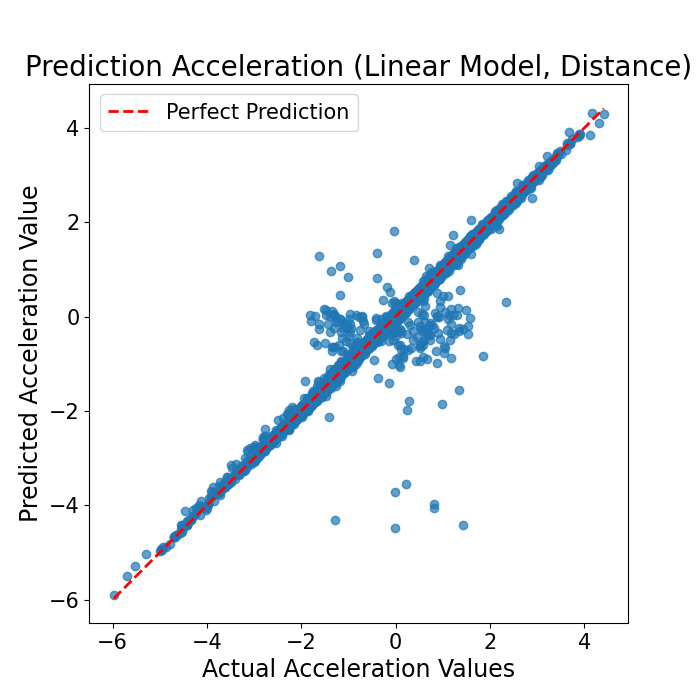
\includegraphics[width=\columnwidth]{images/figures/Prediction Acceleration (Linear Model, Distance).png}
        \caption{Caption for Figure 1}
        \label{fig:minipage3}
    \end{minipage}
    \hfill
    \begin{minipage}[b]{0.45\columnwidth}
        \centering
        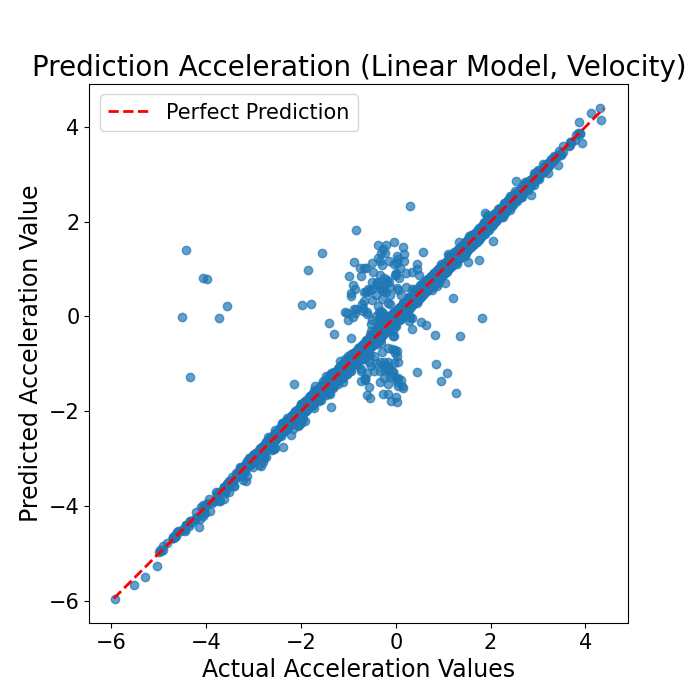
\includegraphics[width=\columnwidth]{images/figures/Prediction Acceleration (Linear Model, Velocity).png}
        \caption{Caption for Figure 2}
        \label{fig:minipage4}
    \end{minipage}
    \caption{Caption for the entire figure}
    \label{fig:combined_figure_2}
\end{figure}


\begin{figure}[t]
    \centering
    \begin{minipage}[b]{0.45\columnwidth}
        \centering
        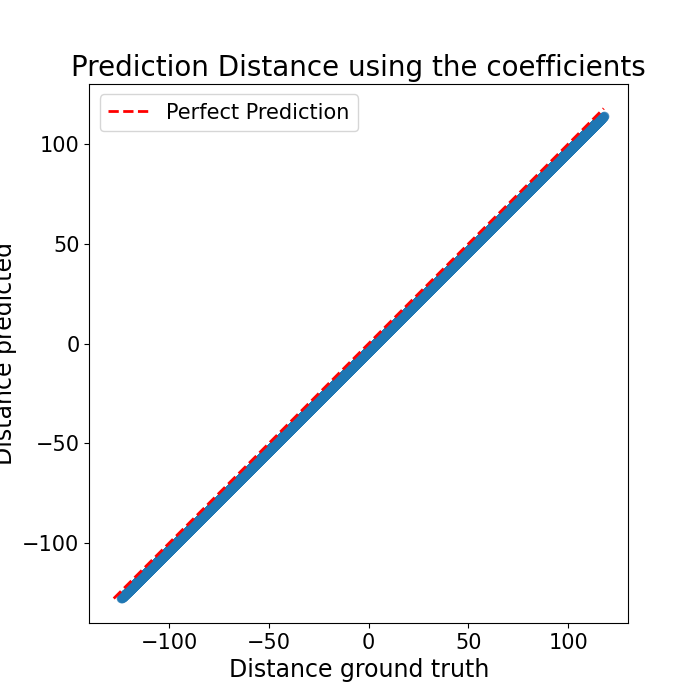
\includegraphics[width=\columnwidth]{images/figures/Prediction Distance using the coefficients.png}
        \caption{Caption for Figure 1}
        \label{fig:minipage3}
    \end{minipage}
    \hfill
    \begin{minipage}[b]{0.45\columnwidth}
        \centering
        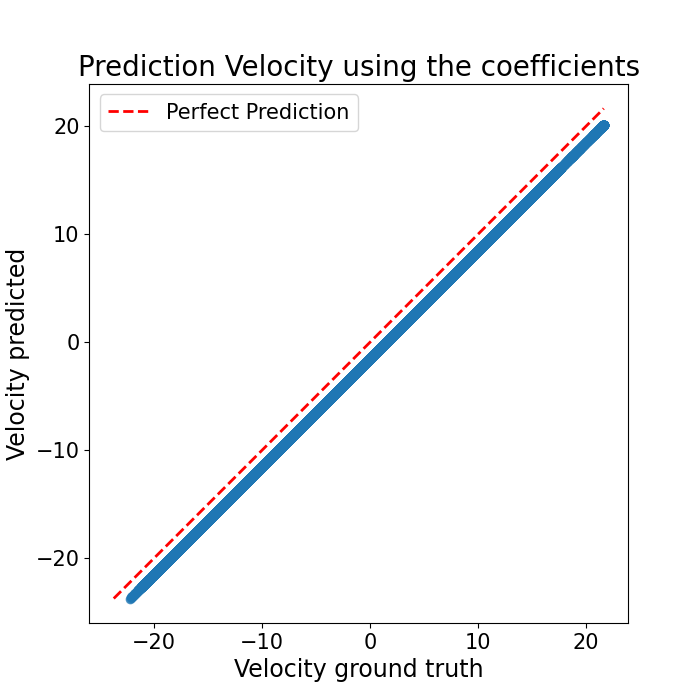
\includegraphics[width=\columnwidth]{images/figures/Prediction Velocity using the coefficients.png}
        \caption{Caption for Figure 2}
        \label{fig:minipage4}
    \end{minipage}
    \caption{Caption for the entire figure}
    \label{fig:combined_figure_2}
\end{figure}


\begin{figure}[t]
    \centering
    \begin{minipage}[b]{0.45\columnwidth}
        \centering
        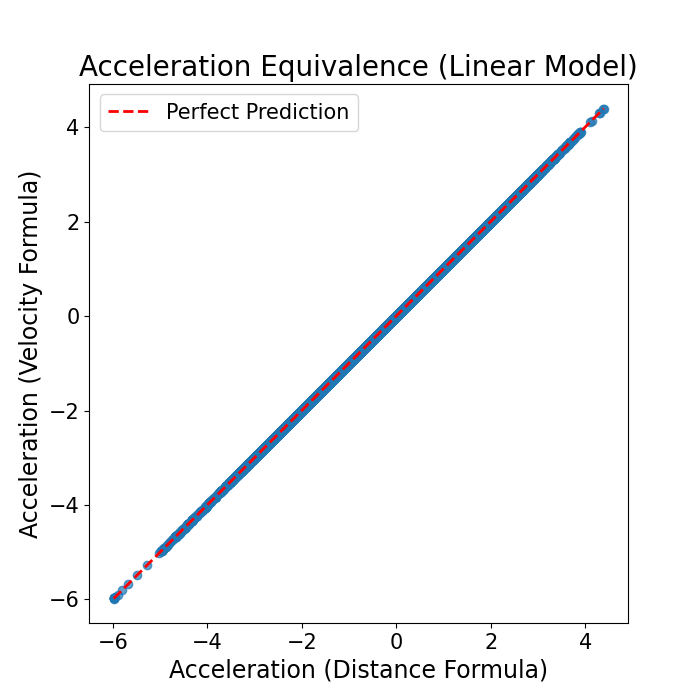
\includegraphics[width=\columnwidth]{images/figures/Acceleration Equivalence (Linear Model).png}
        \caption{Caption for Figure 1}
        \label{fig:minipage3}
    \end{minipage}
    \hfill
    \begin{minipage}[b]{0.45\columnwidth}
        \centering
        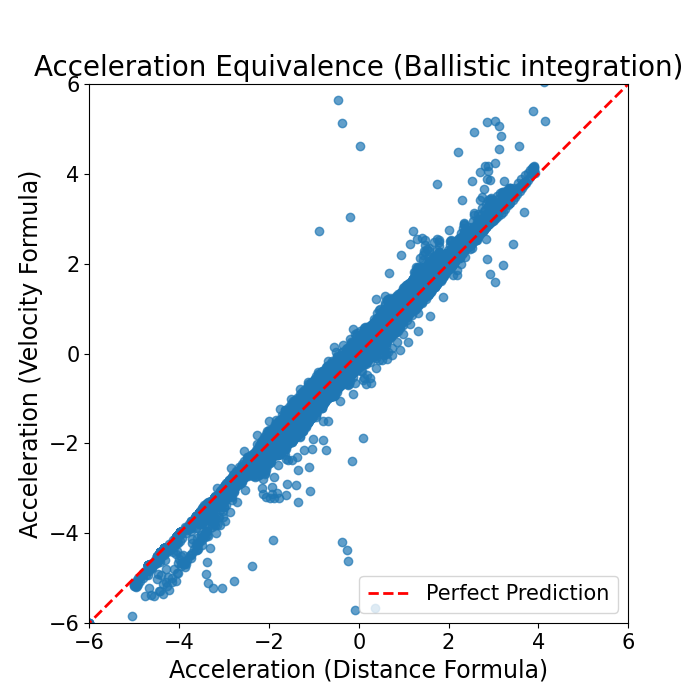
\includegraphics[width=\columnwidth]{images/figures/Acceleration Equivalence (Ballistic integration).png}
        \caption{Caption for Figure 2}
        \label{fig:minipage4}
    \end{minipage}
    \caption{Caption for the entire figure}
    \label{fig:combined_figure_2}
\end{figure}








\subsection{Notable Findings and Observations} 
During the evaluation process, several notable findings were observed. 
Most notably, after rearranging the formula for distance and velocity, a constant error was detected. 
However, increasing the size of NumPy arrays appeared to mitigate this error, indicating a potential 
floating-point precision issue.

\subsection{Future Directions} 
Based on our implementation experience, future research and improvement areas include enhancing the 
precision of NumPy arrays by increasing their size and expanding the dataset to encompass a more extensive
range of scenarios for comprehensive model training and testing.


\section{Conclusion and Future Work}

\subsection{Conclusion}
We demonstrated that our linear model provided us with more equal results for both the distance model and 
the acceleration model.
This highlights the effectiveness of using a linear model as a discrete integration system.
A comparison with the previously used ballistic integration method revealed significantly better performance in terms of accuracy.
Finally, using the coefficients obtained from linear regression, 
we were able to predict both distance and velocity with high accuracy
Although some small error was observed, these results might be sufficient for our neural network.
Visualizations of these predictions showcased their alignment with the ground truth, further validating the effectiveness of our integration model.

\subsection{Future Work}
In future work, we plan to continue refining our integration model to achieve even better results by further fine-tuning its parameters and training procedures. 

Additionally, we aim to explore the integration of our discrete integration model with the neural network developed by the previous team.
By testing the combined model and comparing its effectiveness against the old method, we can gain insights into its actual performance. 

% dunno why this doesnt work
%
% references section

% can use a bibliography generated by BibTeX as a .bbl file
% BibTeX documentation can be easily obtained at:
% http://www.ctan.org/tex-archive/biblio/bibtex/contrib/doc/
% The IEEEtran BibTeX style support page is at:
% http://www.michaelshell.org/tex/ieeetran/bibtex/
%\bibliographystyle{IEEEtran}
% argument is your BibTeX string definitions and bibliography database(s)
%\bibliography{IEEEabrv,../bib/paper}
%
% <OR> manually copy in the resultant .bbl file
% set second argument of \begin to the number of references
% (used to reserve space for the reference number labels box)
\begin{thebibliography}{1}

\bibitem{IEEEhowto:kopka}
H.~Kopka and P.~W. Daly, \emph{A Guide to \LaTeX}, 3rd~ed.\hskip 1em plus
  0.5em minus 0.4em\relax Harlow, England: Addison-Wesley, 1999.

\end{thebibliography}



\bibliographystyle{IEEEtran}
\bibliography{bibliography/social_ai_v1.bib}

% For peer review papers, you can put extra information on the cover
% page as needed:
% \ifCLASSOPTIONpeerreview
% \begin{center} \bfseries EDICS Category: 3-BBND \end{center}
% \fi
%
% For peerreview papers, this IEEEtran command inserts a page break and
% creates the second title. It will be ignored for other modes.
\IEEEpeerreviewmaketitle



% An example of a floating figure using the graphicx package.
% Note that \label must occur AFTER (or within) \caption.
% For figures, \caption should occur after the \includegraphics.
% Note that IEEEtran v1.7 and later has special internal code that
% is designed to preserve the operation of \label within \caption
% even when the captionsoff option is in effect. However, because
% of issues like this, it may be the safest practice to put all your
% \label just after \caption rather than within \caption{}.
%
% Reminder: the "draftcls" or "draftclsnofoot", not "draft", class
% option should be used if it is desired that the figures are to be
% displayed while in draft mode.
%
%\begin{figure}[!t]
%\centering
%\includegraphics[width=2.5in]{myfigure}
% where an .eps filename suffix will be assumed under latex, 
% and a .pdf suffix will be assumed for pdflatex; or what has been declared
% via \DeclareGraphicsExtensions.
%\caption{Simulation Results.}
%\label{fig_sim}
%\end{figure}

% Note that IEEE typically puts floats only at the top, even when this
% results in a large percentage of a column being occupied by floats.


% An example of a double column floating figure using two subfigures.
% (The subfig.sty package must be loaded for this to work.)
% The subfigure \label commands are set within each subfloat command,
% and the \label for the overall figure must come after \caption.
% \hfil is used as a separator to get equal spacing.
% Watch out that the combined width of all the subfigures on a 
% line do not exceed the text width or a line break will occur.
%
%\begin{figure*}[!t]
%\centering
%\subfloat[Case I]{\includegraphics[width=2.5in]{box}%
%\label{fig_first_case}}
%\hfil
%\subfloat[Case II]{\includegraphics[width=2.5in]{box}%
%\label{fig_second_case}}
%\caption{Simulation results.}
%\label{fig_sim}
%\end{figure*}
%
% Note that often IEEE papers with subfigures do not employ subfigure
% captions (using the optional argument to \subfloat[]), but instead will
% reference/describe all of them (a), (b), etc., within the main caption.


% An example of a floating table. Note that, for IEEE style tables, the 
% \caption command should come BEFORE the table. Table text will default to
% \footnotesize as IEEE normally uses this smaller font for tables.
% The \label must come after \caption as always.
%
%\begin{table}[!t]
%% increase table row spacing, adjust to taste
%\renewcommand{\arraystretch}{1.3}
% if using array.sty, it might be a good idea to tweak the value of
% \extrarowheight as needed to properly center the text within the cells
%\caption{An Example of a Table}
%\label{table_example}
%\centering
%% Some packages, such as MDW tools, offer better commands for making tables
%% than the plain LaTeX2e tabular which is used here.
%\begin{tabular}{|c||c|}
%\hline
%One & Two\\
%\hline
%Three & Four\\
%\hline
%\end{tabular}
%\end{table}


% Note that IEEE does not put floats in the very first column - or typically
% anywhere on the first page for that matter. Also, in-text middle ("here")
% positioning is not used. Most IEEE journals/conferences use top floats
% exclusively. Note that, LaTeX2e, unlike IEEE journals/conferences, places
% footnotes above bottom floats. This can be corrected via the \fnbelowfloat
% command of the stfloats package.





% conference papers do not normally have an appendix


% use section* for acknowledgement
% \section*{Acknowledgment}
% The authors would like to thank...





% trigger a \newpage just before the given reference
% number - used to balance the columns on the last page
% adjust value as needed - may need to be readjusted if
% the document is modified later
%\IEEEtriggeratref{8}
% The "triggered" command can be changed if desired:
%\IEEEtriggercmd{\enlargethispage{-5in}}



% references section

% can use a bibliography generated by BibTeX as a .bbl file
% BibTeX documentation can be easily obtained at:
% http://www.ctan.org/tex-archive/biblio/bibtex/contrib/doc/
% The IEEEtran BibTeX style support page is at:
% http://www.michaelshell.org/tex/ieeetran/bibtex/
%\bibliographystyle{IEEEtran}
% argument is your BibTeX string definitions and bibliography database(s)
%\bibliography{IEEEabrv,../bib/paper}
%
% <OR> manually copy in the resultant .bbl file
% set second argument of \begin to the number of references
% (used to reserve space for the reference number labels box)

% that's all folks
\end{document}


